\lstset {
tabsize=2,
basicstyle=\footnotesize\ttfamily,breaklines=true
}

\section{Abstracción y modelado}
	El objeto a modelar es una intersección de $N$ calles o avenidas. Con el objeto de profundizar el análisis, se tomará el caso de una intersección de dos avenidas, como la que se puede ver en la figura \ref{fig:interseccion-base}. A lo largo de este trabajo se utilizará el término \enquote{tramo} para designar al medio por el cual arriban vehículos o personas a la intersección.
	
	Una avenida de doble sentido de circulación tiene dos tramos. Con lo cual una intersección de dos avenidas tiene cuatro tramos más un tramo diferenciado para los peatones. 
	\begin{figure}[htbp]
	\centering
	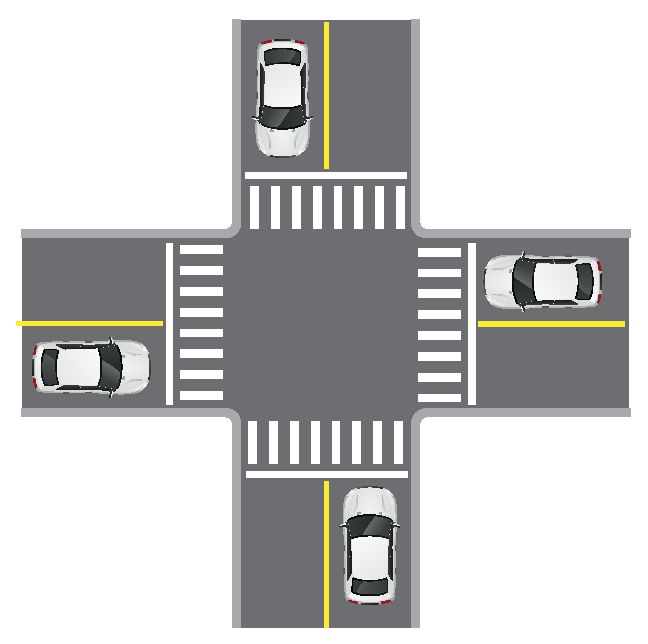
\includegraphics[width=6cm]{imagenes/interseccion-base.eps}
	\caption{Intersección base.}
	\label{fig:interseccion-base}
	\end{figure}
	Se asume que existe una forma fiable de detectar la presencia de vehículos en un tramo.

	Se dice que un tramo está \enquote{activo} si y solo si hay al menos un vehículo en él.

	Por otro lado, también se debe tener en cuenta la presencia de peatones. Para ello se asume que en cada senda peatonal de la intersección hay un pulsador que permite a un peatón solicitar el paso por una de las sendas peatonales. El tramo de peatones se activa con presionar una vez el pulsador y permanece activo hasta ser atendido.

	Se dice que un tramo es atendido cuando el sistema de semáforos permite el paso de vehículos o personas, es decir, tiene su semáforo correspondiente en verde. Para simplificar el análisis, se modela a la intersección como un recurso compartido al cual se accede con exclusión mutua. Es decir, la intersección puede ser adquirida a lo sumo por un tramo.



	\subsection{Especificación del comportamiento}\label{sec:spec}

		Para entender mejor el problema a resolver se analiza cada situación que se presenta en una intersección.
		A continuación se detalla cada caso y se describa la forma en la que se espera que el programa responda.



	\subsection{Ningún tramo activo}

		Cuando no hay ningún tramo activo, es decir, no hay vehículos en ninguna línea de detención, el sistema debe dar paso a todos los tramos de forma periódica y de a turnos (\emph{round-robin}).
		Se puede ver esta situación en la figura \ref{fig:ningun-activo}.

		Si estuviera activo el tramo del peatón, entonces se incluye al tramo de peatón al conjunto de tramos participantes del \emph{round-robin}.

		\begin{figure}[htbp]
			\centering
			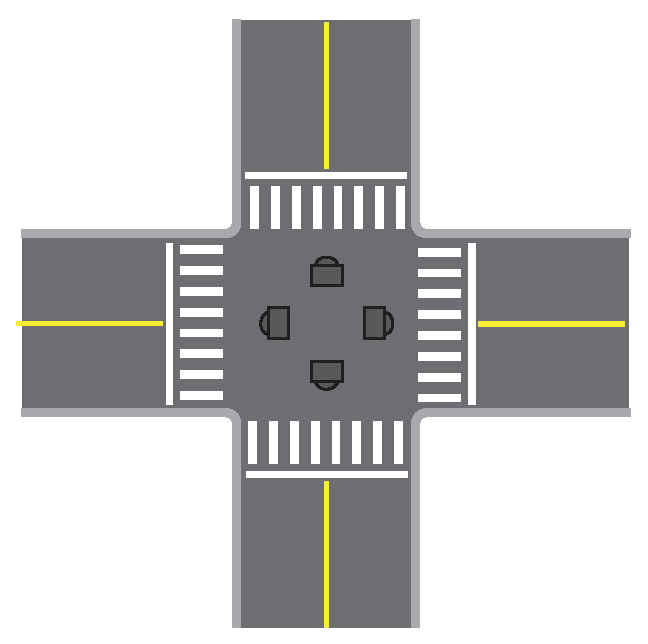
\includegraphics[width=6cm]{imagenes/ningun-activo.eps}
			\caption{Intersección sin vehículos ni peatón.}
			\label{fig:ningun-activo}
		\end{figure}



	\subsection{Un tramo activo}

		Cuando hay un solo tramo activo, entonces se le debe dar el paso ininterrumpidamente hasta que haya otro tramo activo (esto incluye el caso en que se active el tramo de peatones).
		Se puede ver la situación de estar un sólo tramo activo en la figura \ref{fig:un-activo}.

		\begin{figure}[htbp]
			\centering
			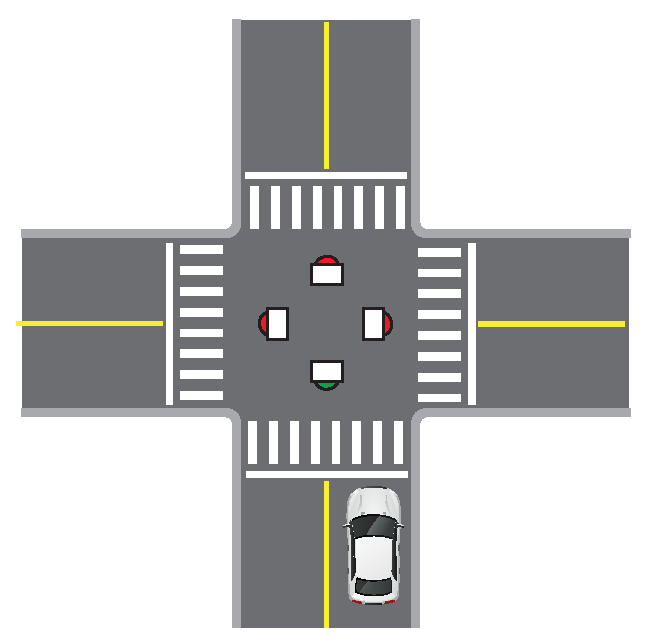
\includegraphics[width=6cm]{imagenes/un-activo.eps}
			\caption{Intersección con un tramo activo.}
			\label{fig:un-activo}
		\end{figure}



	\subsection{Más de un tramo activo}

		Cuando hay mas de un tramo activo, simplemente debe hacerse \emph{round-robin} como en el caso anterior pero sólo participan los semáforos correspondientes a los tramos activos, permanenciendo el resto en rojo.
		Se puede ver la situación de estar dos tramos activos en la figura \ref{fig:dos-activos}.

		\begin{figure}[htbp]
			\centering
			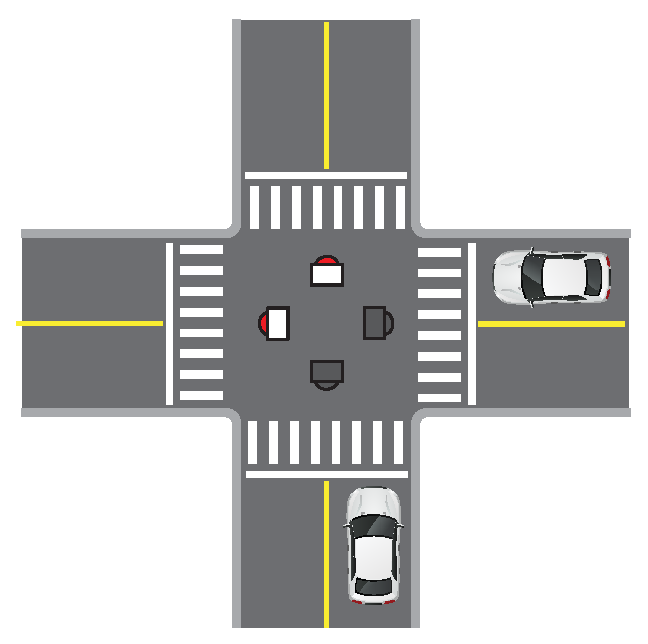
\includegraphics[width=6cm]{imagenes/dos-activos.eps}
			\caption{Intersección con dos tramos activos.}
			\label{fig:dos-activos}
		\end{figure}

		A modo de resumen, se lista las situaciones y el comportamiento correspondiente en la tabla \ref{tab:comportamiento}.

		\rowcolors{2}{gray!25}{white}
		\begin{table}[htbp]
			\centering
			\caption{Resumen de comportamiento del sistema ante distintas combinaciones de entrada.}
			\vspace{0.25cm}
			\label{tab:comportamiento}
			\begin{tabular}{cc}
				\toprule
				\bf{Tramos activos} & \bf{Comportamiento} \\
				\midrule
				0 & \emph{round-robin} entre todos los tramos. \\
				1 & Verde ininterrumpido al único tramo activo. \\
				$1 < \mbox{TA} \le N$ & \emph{round-robin} entre los tramos activos. \\
				$N$ & \emph{round-robin} entre todos los tramos activos. \\
				\bottomrule
			\end{tabular}
		\end{table}



	\subsection{Interacción con peatones}

		En caso de que haya peatones esperando por cruzar, entonces los mismos deben establecer un pedido al sistema, presionando el botón que se encuentra al costado de cada semáforo.
		Esta acción les garantiza que en algún momento todos los semáforos pondrán sus luces en rojo, evitando que cualquier auto cruce y se encienda la luz blanca del peatón.
		En ese momento cualquier peatón que se encuentre en alguna de las esquinas tendrá paso durante un tiempo.

		Al finalizar ese lapso, se vuelve al funcionamiento normal, previamente descripto.
		En caso de que hubiera más peatones por cruzar, el sistema no les volverá a otorgar paso hasta que el botón no sea presionado nuevamente.
		Esta es la única diferencia entre los semáforos de los autos y de los peatones.

		En la figura \ref{fig:peaton-activo} se observa cómo interactúan los peatones con el sistema de semáforos previamente descripto.

		\begin{figure}[htbp]
			\centering
			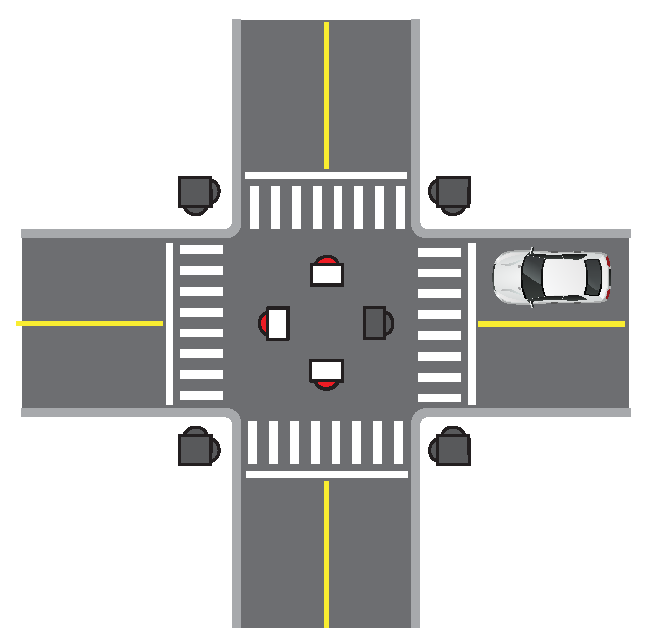
\includegraphics[width=6cm]{imagenes/peaton-auto.eps}
			\caption{Intersección con un tramo y el tramo de peatón activos.}
			\label{fig:peaton-activo}
		\end{figure}



	\subsection{Uso de procesos}\label{sec:proc}

		Basándose en el marco teórico de la programación concurrente, se puede modelar a cada tramo como un proceso que trata de acceder al recurso compartido (la intersección).
		De esta forma el problema del control del tránsito se reduce al de la planificación de un recurso compartido.
		Este recurso compartido programáticamente se convierte entonces en una sección crítica.



\section{Implementación del sistema y resultados}

	La implementación del controlador de semáforos se realizó sobre un Arduino Uno, utilizando la plataforma de desarrollo Arduino.
	Como herramienta de desarrollo se utilizó la extensión PlatformIO para el editor de texto Visual Studio Code.

	FreeRTOS provee proyectos prearmados y preconfigurados para tomar como código base y realizar el desarrollo directamente sobre ellos.
	No existe una implementación oficialmente soportada por Real Engineers Ltd. (la empresa detrás de FreeRTOS), ni tampoco una implementación para el microcontrolador del Arduino Uno, el Atmega 328P.
	Sin embargo, existe una implementación no oficialmente soportada para Arduino Uno (ver sección \ref{sec:bib}).
	

	Se realizaron tres implementaciones que implementan el sistema según lo especificado en la sección \ref{sec:spec}.
	Cada implementación hace uso de las distintas funcionalidades provistas por FreeRTOS de forma distinta, pero todas tienen en común el uso de semáforos, mútexes y tareas.
	Los procesos se traducen a tareas en FreeRTOS y la exclusión mutua perteneciente a la sección crítica mencionada en la sección \ref{sec:proc} se hace cumplir con el uso de semáforos y mútexes.



	\subsection{Implementación A}

	En esta primera implementación, se modela a cada semáforo como una tarea de FreeRTOS y sus prioridades son fijas.
	Adicionalmente existe un proceso controlador, de máxima prioridad, que determina quién es la próxima tarea en ingresar a la sección crítica, es decir, en poner en verde su semáforo.

	El controlador realiza dicha planificación a partir de los datos sensados por una tarea sensor que lee la actividad de cada tramo.
	Ésta tiene una prioridad también alta, pero solo corre cuando el controlador le indica, utilizándose un semáforo para la comunicación.

	Al obtener los datos, éste se los pasa al controlador, quien permanece a la espera de los mismos, mediante el modelo productor/consumidor.
	Esta solución representa una utilización ineficiente de los recursos ya que periódicamente se realiza una copia de los datos obtenidos para que el controlador pueda disponer de los datos.

	El controlador toma los datos y realiza una lista de ejecución que determina en qué orden deben ejecutarse las tareas.
	Cada tarea se duerme en su propio semáforo, a pesar de que la intersección sea compartida.
	Se utiliza un semáforo para esperar a poner la luz en verde y otro para ponerla en rojo.

	El controlador ejecuta los \code{V\(\)} de cada uno, según corresponda.

	Entre las ventajas de esta implementación se encuentra el hecho de que se tiene un control total de las ejecuciones de cada proceso.
	Sin embargo, esta implementación requiere de un esfuerzo adicional para hacer \emph{round-robin} cuando todos los semáforos tienen sus tramos inactivos. En el momento de desarrollo esto no implicaba un problema porque no estaba específicado que deba manejarse este caso. Pero se consideró que esta situación debería ser contemplada y se modificó la especificación para la siguiente implementación.

	El pseudo código de la tarea controlador se puede observar en el código \ref{lst:imp-a}.

	\begin{lstlisting}[float, label=lst:imp-a, caption=Pseudocódigo de la tarea controlador.]
		while (true)
			Rojo()
			P(verdeSem)
			Verde()
			Delay(...)
			P(rojoSem)
			Amarillo()
			Delay(...)
		Fin while
	\end{lstlisting}



	\subsection{Implementación B}

	En esta implementación se trata de transferir hacia el kernel de FreeRTOS la responsabilidad de elegir cuál semáforo adquiere el recurso, es decir, a cuál tramo se le da el paso.
	Se elimina la tarea controlador que planificaba el acceso al medio y se deja total libertad al scheduler de FreeRTOS.
	Sin embargo, para representar la actividad de cada tarea se cuenta con un sistema de prioridades dinámicas.
	De esta forma, el scheduler de FreeRTOS sabe en todo momento cuáles semáforos tienen autos en sus tramos y cuáles no.

	Se utilizan dos valores de prioridad en las tareas, una alta y una baja.
	Las tareas correspondientes a tramos activos toman una prioridad alta y las tareas correspondientes a tramos inactivos toman una prioridad baja. 
	La prioridad de las tareas está ligada a la actividad de su tramo, con lo cual las prioridades van variando a lo largo del funcionamiento del sistema.

	Al igual que en la implementación A, se tiene, $N + 1$ ($N$ tramos y el tramo distinguido para los peatones) tareas, donde cada una representa un tramo y todas tratan de acceder a una sección crítica, protegida por un sólo mútex.

	Para que el orden en el cual cada tarea adquiere el mútex sea determinístico, no es suficiente que el planificador sea débilmente \emph{fair}, sino que es necesario que se aplique una política de planificación que realice \emph{round-robin} entre tareas de misma prioridad.
	FreeRTOS permite lograr esto mediante su archivo de configuración.

	En esta implementación se utiliza el modo cooperativo de planificación que ofrece FreeRTOS, de forma que al final de cada ejecución se cede el control de la CPU hacia otra tarea de forma explícita.

	Cada tarea realiza el algoritmo mostrado en el código \ref{lst:imp-b}.

	\begin{lstlisting}[float, label=lst:imp-b, caption=Pseudocódigo del programa que corre cada tarea en la implementación B.]
		while (true)
			P(mutex)
			do
				Verde()
				Delay(...)
				Leer sensores y actualizar prioridades
			while (Este tramo sea el unico activo)
			Amarillo()
			Delay(...)
			Rojo()
			Delay(...)
			V(mutex)
			yield()
		Fin while
	\end{lstlisting}

	En la figura \ref{lst:imp-b} se observa una función \code{yield\(\)} que se encarga de ceder la CPU hacia otra tarea de mayor o igual prioridad.
	En caso de que no existiera tal tarea, le vuelve a tocar a la tarea que ejecuto dicha función.

	\subsubsection{Problema del cambio de la prioridad}
	El principal inconveniente de esta implementación se encuentra en el uso de prioridades variantes en el tiempo combinado con tareas que no están listas para ejecutarse.

	En la implementación de FreeRTOS de Arduino, cambiar la prioridad de tareas que están bloqueadas (en este caso, en un semáforo), tiene el efecto inesperado de que no se utilizan las nuevas prioridades en el próximo cambio de contexto, sino en el que le sigue a esto. Este hecho rompe la lógica del algoritmo de esta implementación.

	Se intentó resolver este problema con una modificación en el algoritmo: en vez de simplemente cambiar las prioridades, primero se hizo que la tarea que se cambie su prioridad a una prioridad mayor (estricto) a todas las otras, $P_{max}$.
	Esto se hace para que al cambiar las prioridades de todas las tareas, nunca pierda el control la tarea que realiza el cambio.
	Luego, hace \code{V\(\)} sobre el semáforo que tienen todas las tareas en común, para que pasen a la cola \emph{ready to run}, para evitar el error mencionado anteriormente.
	Una vez que tiene esta prioridad máxima, procede a hacer el cambio de las prioridades, sin cambiar la suya.
	Antes de establecer su prioridad al valor correspondiente, hace \code{P\(\)}, sobre el semáforo en común, para retornarlo al estado en que estaba.

	Dicha modificación tampoco produjo los resultados esperados cuando se ejecutaba sobre Arduino.
	Para investigar si se trata de un problema en la implementación de FreeRTOS para Arduino, se escribió un pequeño programa utilizando una implementación de FreeRTOS para Win32, con lo que se puede simular la planificación de tareas directamente en Windows.

	Este programa crea cuatro tareas: $T_1$, $T_2$, $T_3$ y $T_4$. Existe un semáforo $S$ inicializado en 1.
	Cada tarea $T_i$ compite por tomar $S$, cuando lo hace, imprime su nombre, espera un segundo, y si se hicieron dos vueltas en el \emph{round-robin}, cambia las prioridades como se describió anteriomente. Se puede ver el pseudocódigo del programa implementado en el código \ref{lst:win32}. \code{NuevasPrioridades} es un arreglo con nuevas prioridades que provienen de un arreglo de arreglos previamente definido. La primera entrada en este arreglo de arreglos es un set de prioridades todas iguales, de manera que el primer \emph{round-robin} ejecute las tareas en orden creciente.

	\begin{lstlisting}[float, label=lst:win32, caption=Pseudocódigo del programa escrito para FreeRTOS-Win32.]
	N := 0
	Tarea[i = 1 .. 4]
		P(S)
		ImprimirNombre(i)
		Delay(1 s)
		if N = 8 {
			CambiarPrioridad(Tarea[I], MAXIMA)
			Tarea[j].Prioridad = MAXIMA
			V(S)
			for j = 1 to 4 {
				if (j != i)
					Tarea[j].Prioridad = NuevasPrioridades[j]
			}
			P(S)
			Tarea[i].Prioridad = NuevasPrioridades[i];
			N = 0
		}
	}
	\end{lstlisting}

	Se puede ver parte de la salida de este programa en el código \ref{lst:output-win32}. Allí se muestran únicamente el comienzo del programa y luego otro momento de la ejecución. Se puede ver que inicialmente las tareas obtienen el semáforo en el orden esperado. Sin embargo, despues de probar varias combinaciones distintas, al volver a utilizar las mismas prioridades, se ejecutan las mismas tareas pero en un orden distinto, que no es lo que se quería lograr en el sistema.

	Este problema fue el que indicó que no se podría realizar el sistema acorde a la especificación propuesta con esta técnica (prioridades cambiantes), ya que esta fuera del alcance del equipo este aspecto del planificador de FreeRTOS.

	\begin{lstlisting}[float, label=lst:output-win32, caption=Salida del programa de prueba escrito para Win32.]
		Task 1
		Task 2
		Task 3
		Task 4
		Task 1
		Task 2
		Task 3
		Task 4
		-----------
		....
		-----------
		Task 1
		Task 3
		Task 2
		Task 1
		Task 3
		Task 2
		Task 1
		Task 3
	\end{lstlisting}

	Este problema tuvo como consecuencia que se abandonara esta implementación y se pensara en una nueva donde las prioridades fuesen fijas.



	\subsection{Implementación C}
	La tercera implementación de este proyecto surge con la necesidad de eliminar los problemas que se introducen en las anteriores soluciones.
	El principal inconveniente que se busca solucionar, se relaciona con el uso de las prioridades variantes en el tiempo.
	En particular, cuando se le cambia la prioridad a una tarea que se encuentra en el estado bloqueada, el programa no responde tal como era de esperarse.

	Para esta implementación se sigue modelando a cada tramo como una tarea de FreeRTOS (incluyendo al de los peatones) y se toma las mejores características de los anteriores diseños.
	En primer lugar, las prioridades vuelven a ser estáticas, evitando así el problema del cambio de prioridades sobre tareas que no se encuentren en estado \emph{ready to run} ni \emph{running}.

	Por otra parte, se elimina la existencia de un proceso controlador.
	La tarea de planificación queda a cargo del kernel de FreeRTOS.
	De esta forma el diseño de la solución queda más simple, tal como en la segunda implementación.
	No se utilizan búffers, ni el modelo productor/consumidor y los recursos se aprovechan al máximo.

	Es fácil de extender a más tramos, por ejemplo si se agrega el cruce con un diagonal.
	Además permite pensar al peatón como un semáforo más, cosa que no ocurría en la primera implementación.

	La principal diferencia respecto de las anteriores soluciones es que en este diseño, la intersección no se implementa con un único mútex.
	Cabe destacar que se sigue pensando como una sóla sección crítica pero en su codificación representa un mútex por cada tarea.

	De esta forma cada proceso se duerme en su propio mútex e independientemente de la actividad que haya en su tramo, se garantiza que en algún momento entra a la sección crítica.
	Cuando dicho evento ocurre, la tarea tiene posibilidad de consultar con su sensor si hay autos o peatones (según corresponda) esperando por cruzar, y en caso afirmativo, coloca verde en su semáforo.

	Al finalizar su trabajo, la tarea despierta a la próxima para que tenga posibilidad de ejecutarse, y la primera se vuelve a dormir en su propio mútex nuevamente hasta que le toque correr otra vez.

	Este diseño permite que las tareas se autocontrolen sin la necesidad de la existencia de un proceso controlador.
	La técnica utilizada se conoce como \emph{passing the baton}.

	Cada tarea realiza el algoritmo explicitado en el código \ref{lst:imp-c}.

	\begin{lstlisting}[float, label=lst:imp-c, caption=Pseudocódigo del programa que corre cada tarea en la implementación C.]
		int i = id;

		while (true)
			P(mutex[i])
			if (es activo o no hay activos)
				do
					Verde()
					Delay(...)
					Leer sensores
				while (Este tramo sea el unico activo)
				Amarillo()
				Delay(...)
				Rojo()
				Delay(...)
			V(mutex[i + 1])
		Fin while
	\end{lstlisting}

	En la figura \ref{lst:imp-c} se observa como cada tarea se duerme en su propio mutex $i$ y al finalizar su ejecución despierta al semáforo $i+1$.



\section{Conclusiones}\label{sec:conclusiones}
	En este trabajo se analizaron distintas formas de implementar un sistema de semáforos inteligentes sujeto a la especificación aquí dada. Las principales conclusiones involucran a FreeRTOS y estas son: el orden en que se despiertan las tareas dormidas en un semáforo binario no está especificado por el planificador, con lo que su comportamiento está ligado a la implementación y no se puede fiar de el. Posiblemente exista un error en la implementación de FreeRTOS para Arduino que retrasa los efectos esperados al cambiar prioridades de tareas bloqueadas.

	Estos hechos tienen como consecuencia el hecho de que no es fehacible implementar un sistema conforme a la especificación dada utilizando el planificador de un kernel como el de FreeRTOS de la manera realizada en la implementación B.

